%%%%%%%%%%%%%%%%%%%%%%%%%%%%%%%%%%%%%%%%%
% Arsclassica Article
% LaTeX Template
% Version 1.1 (10/6/14)
%
% This template has been downloaded from:
% http://www.LaTeXTemplates.com
%
% Original author:
% Lorenzo Pantieri (http://www.lorenzopantieri.net) with extensive modifications by:
% Vel (vel@latextemplates.com)
%
% License:
% CC BY-NC-SA 3.0 (http://creativecommons.org/licenses/by-nc-sa/3.0/)
%
%%%%%%%%%%%%%%%%%%%%%%%%%%%%%%%%%%%%%%%%%

%----------------------------------------------------------------------------------------
%	PACKAGES AND OTHER DOCUMENT CONFIGURATIONS
%----------------------------------------------------------------------------------------

\documentclass[
10pt, % Main document font size
a4paper, % Paper type, use 'letterpaper' for US Letter paper
oneside, % One page layout (no page indentation)
%twoside, % Two page layout (page indentation for binding and different headers)
headinclude,footinclude, % Extra spacing for the header and footer
BCOR5mm, % Binding correction
]{scrartcl}

%%%%%%%%%%%%%%%%%%%%%%%%%%%%%%%%%%%%%%%%%
% Arsclassica Article
% Structure Specification File
%
% This file has been downloaded from:
% http://www.LaTeXTemplates.com
%
% Original author:
% Lorenzo Pantieri (http://www.lorenzopantieri.net) with extensive modifications by:
% Vel (vel@latextemplates.com)
%
% License:
% CC BY-NC-SA 3.0 (http://creativecommons.org/licenses/by-nc-sa/3.0/)
%
%%%%%%%%%%%%%%%%%%%%%%%%%%%%%%%%%%%%%%%%%

%----------------------------------------------------------------------------------------
%	REQUIRED PACKAGES
%----------------------------------------------------------------------------------------

\usepackage[ nochapters, % Turn off chapters since this is an article
beramono, % Use the Bera Mono font for monospaced text (\texttt)
eulermath,% Use the Euler font for mathematics 
pdfspacing, % Makes use of pdftex’ letter spacing capabilities via the microtype package
dottedtoc % Dotted lines leading to the page numbers in the table
%          ofcontents 
]{classicthesis} % The layout is based on the Classic Thesis style

\usepackage{arsclassica} % Modifies the Classic Thesis package

\usepackage[T1]{fontenc} % Use 8-bit encoding that has 256 glyphs

\usepackage[utf8]{inputenc} % Required for including letters with accents

\usepackage{graphicx} % Required for including images
\graphicspath{{Figures/}} % Set the default folder for images

\usepackage{enumitem} % Required for manipulating the whitespace between and within lists

\usepackage{lipsum} % Used for inserting dummy 'Lorem ipsum' text into the template

\usepackage{subfig} % Required for creating figures with multiple parts (subfigures)

\usepackage{amsmath,amssymb,amsthm} % For including math equations, theorems, symbols, etc

\usepackage{varioref} % More descriptive referencing

\usepackage{enumitem}

%----------------------------------------------------------------------------------------
%	THEOREM STYLES
%---------------------------------------------------------------------------------------

\theoremstyle{definition} % Define theorem styles here based on the definition style (used for definitions and examples)
\newtheorem{definition}{Definition}

\theoremstyle{plain} % Define theorem styles here based on the plain style (used for theorems, lemmas, propositions)
\newtheorem{theorem}{Theorem}

\theoremstyle{remark} % Define theorem styles here based on the remark style (used for remarks and notes)

%----------------------------------------------------------------------------------------
%	HYPERLINKS
%---------------------------------------------------------------------------------------

\hypersetup{
%draft, % Uncomment to remove all links (useful for printing in black and white)
colorlinks=true, breaklinks=true, bookmarks=true,bookmarksnumbered,
urlcolor=webbrown, linkcolor=RoyalBlue, citecolor=webgreen, % Link colors
pdftitle={}, % PDF title
pdfauthor={\textcopyright}, % PDF Author
pdfsubject={}, % PDF Subject
pdfkeywords={}, % PDF Keywords
pdfcreator={pdfLaTeX}, % PDF Creator
pdfproducer={LaTeX with hyperref and ClassicThesis} % PDF producer
} % Include the structure.tex file which specified the document structure and layout

\hyphenation{Fortran hy-phen-ation} % Specify custom hyphenation points in words with dashes where you would like hyphenation to occur, or alternatively, don't put any dashes in a word to stop hyphenation altogether

%% additional packages:
\usepackage{wrapfig}
\usepackage[left=1.5in,right=1in,top=1in,bottom=1in]{geometry}
\usepackage{caption}

%----------------------------------------------------------------------------------------
%	TITLE AND AUTHOR(S)
%----------------------------------------------------------------------------------------

\title{
\includegraphics[width=5cm]{Figures/datarea.pdf} \\
{\large \#SummerDataChallenge}} % The article title

\author{ {\large Benjamin L. Moore\textsuperscript{1}}} % The article author(s) - author affiliations need to be specified in the AUTHOR AFFILIATIONS block

\date{} % An optional date to appear under the author(s)

%----------------------------------------------------------------------------------------

% custom macros:

\newcommand*{\logo}{
\includegraphics[scale=.22]{Figures/datarea.pdf}}

\begin{document}

%----------------------------------------------------------------------------------------
%	HEADERS
%----------------------------------------------------------------------------------------

\renewcommand{\sectionmark}[1]{\markright{\spacedlowsmallcaps{summerdatachallenge}}} % The header for all pages (oneside) or for even pages (twoside)
%\renewcommand{\subsectionmark}[1]{\markright{\thesubsection~#1}} % Uncomment when using the twoside option - this modifies the header on odd pages
\lehead{\mbox{\llap{\small\thepage\kern1em\color{halfgray} \vline}\color{halfgray}\hspace{0.5em}\rightmark\hfil}} % The header style

\pagestyle{scrheadings} % Enable the headers specified in this block

%----------------------------------------------------------------------------------------
%	TABLE OF CONTENTS & LISTS OF FIGURES AND TABLES
%----------------------------------------------------------------------------------------

\maketitle % Print the title/author/date block

\setcounter{tocdepth}{2} % Set the depth of the table of contents to show sections and subsections only

% \tableofcontents % Print the table of contents

% \listoffigures % Print the list of figures

% \listoftables % Print the list of tables

%----------------------------------------------------------------------------------------
%	ABSTRACT
%----------------------------------------------------------------------------------------
\vspace{-4em}
\section*{Overview} 

I analysed the {\bf London house prices} dataset is several innovative
ways. Firstly \emph{fractal context} shows how house sales within an
arbitrary area relate to those if neighbouring districs, up and down
the postcode hierarchy. Secondly, I employed \emph{ARIMA forecasting}
to extrapolate an area's price trend with an eye to suggesting
profitable investments. Finally, these and other metrics were combined
into an \emph{investment grade} for a given postcode area. Combined
this set of analyses forms the basis of \logo, a product aimed at
``democratising real estate investment'', offering individuals and
businesses quantitative insights for data-driven investment
decisions. 

A fully-featured report is online at {\bf \href{http://blm.io/datarea}{blm.io} }and
scripts to reproduce all analyses are available from
{\bf \href{http://github.com/blmoore/summerdatachallenge}{github}}.

%----------------------------------------------------------------------------------------
%	AUTHOR AFFILIATIONS
%----------------------------------------------------------------------------------------

{\let\thefootnote\relax\footnotetext{\textsuperscript{1} \textit{MRC
      Human Genetics Unit, University of Edinburgh, Scotland, United Kingdom}}}

%----------------------------------------------------------------------------------------

%\newpage % Start the article content on the second page, remove this if you have a longer abstract that goes onto the second page

%----------------------------------------------------------------------------------------
%	INTRODUCTION
%----------------------------------------------------------------------------------------

\section{Description of analyses}

When considering a property in a given area, you may ask a realtor
questions like, how do prices here compare to surrounding postcodes?
How have prices increased over time? 

\setlength{\intextsep}{.1em}
\begin{wrapfigure}{R}{.45\textwidth}
\begin{center}
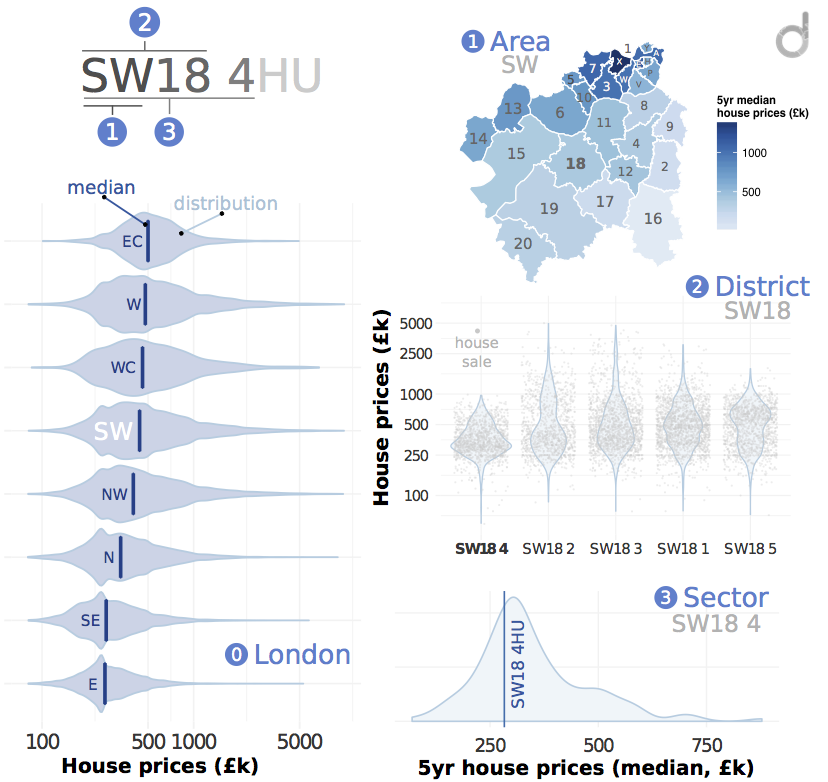
\includegraphics[width=.44\textwidth]{Figures/fractal.png}
\caption{ Fractal context of postcode SW18 4HU in Wandsworth, South London.}
\end{center}
\end{wrapfigure}

A real estate professional can give an opinion based on anecdotal
evidence and the limited sample size they have experienced, but with a
large dataset we can address these questions quantitatively and
present them as clear visualisations.

\subsection{Fractal context}

Letting and sales sites may currently list some recent sales, but it's
not currently possible to see a quantitative overview of property
prices in a region, within the context of its sector, district and
postcode.

These questions can be answered with a clear and intuitive data
visualisation of price distributions in the postcode hierarchy --- we
call this the fractal context of a property price.

\subsection{ARIMA forecasting}

Given area price histories, it's of interest to investors to speculate
on potential investment returns for a given property area. This can be
done through time series analysis using the autoregressive integrated
moving average (ARIMA) model. Investment returns can be maximised by
selecting areas with maximal growth
projections.\textsuperscript{$\star$} \\

\begin{figure}[h]
\begin{center}
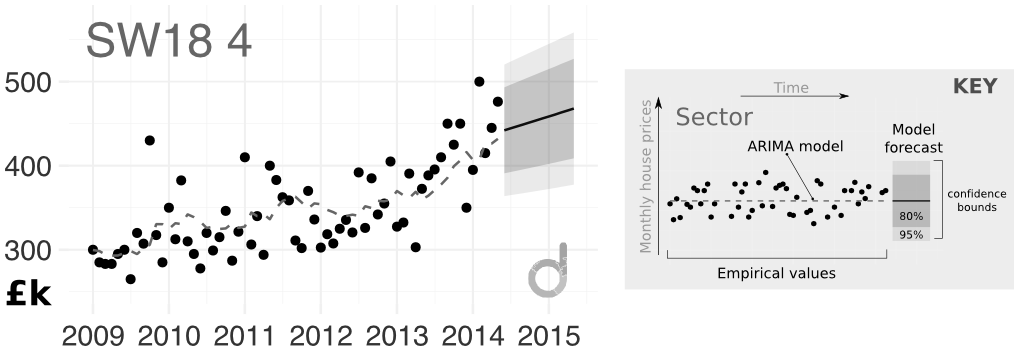
\includegraphics[width=.9\textwidth]{Figures/arima.png}
\caption{Example ARIMA forecast of median house prices for a specific postcode.}
\end{center}
\end{figure}

\vspace{-2em}
\subsection{Investment grading}

Combining growth forecasts and contextual information, as well as
other derived metrics from this dataset, allow an approximate
investment grading, relative to other postcodes within the area
covered by this dataset. This intuitive output metric can help
prioritise areas ripe for property investment. \\

{\let\thefootnote\relax\footnotetext{\textsuperscript{$\star$}
    Data intended to assist investors and does not constitute
    investment advice; independent advice should be sought where appropriate. }}

%----------------------------------------------------------------------------------------
%	METHODS
%----------------------------------------------------------------------------------------
\vspace{-2em}
\section{Value generation}

\logo \hspace{.1em} would first be released as both a web service and
associated apps for mobiles and tablets. These would offer limited
analysis and visualisation for free, with user analytics and feedback
helping to validate the business model.

\begin{wrapfigure}{r}{.4\textwidth}
\begin{center}
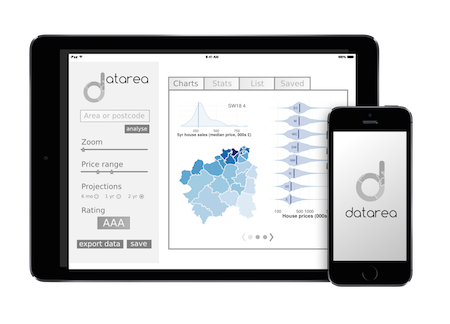
\includegraphics[width=.39\textwidth]{Figures/mockup.png}
\caption{ iOS app mock-up.}
\end{center}
\end{wrapfigure}

A small data science team could expand analyses, integrating novel
public and privately-acquired datasets and release them under a
rolling subscription model, aimed at private landlords and property
speculators, as well as professional real estate investment trusts
(REITs). Significant revenue could be generated through tailored
partnerships with funds and high net-worth individuals.

Should the product not succeed in a direct-to-consumer market, the
business could pivot to an analytics provider for existing letting and
sales sites, offering unique data insights indirectly to the consumer
market, or as independent fund consultants for the financial
services. Having produced a functional product positions \logo \hspace{.1em} to
succeed in innovative real estate analytics.

\begin{flushright}
{\small Full version online at: \href{http://blm.io/datarea}{blm.io/datarea}}
\end{flushright}

\begin{figure}[h!]
\begin{center}

\includegraphics[width=.1\textwidth]{Figures/logo.png} \\

\includegraphics[scale=.4]{Figures/datarea.pdf} \\
\caption*{ {\sf Democratising real estate investment}}
\end{center}
\end{figure}

\end{document}